\section{Documentation}

\subsection{Context and Terms}
The position of the sun from perspective of an observer is defined by two parameters:

\begin{itemize}
  \item the azimuth $\Theta$, which tells the observer, how far (in degree) he must turn around from the North direction,
  \item the altitude $\phi$, which tells the observer, how height (in degree) about the horizon he must look to see the sun.
\end{itemize}
The azimuth can take a value in the interval $[0,360)$. 
The altitude can take a value in the interval $[0,90]$, whereas 0 is the horizon, 90 is the zenith.
We do not care so much about how far is the sun, so we normalize this distance to 1.


The figure~\ref{fig:hz-coordinate} shows these parameter. 
The coordinate system, which takes the position of the observer as the centre, 
and the observer's local horizon as the  fundamental plane,
is called horizontal coordinate system.\footnote{dt.: topozentrisches Koordinatensystem}

\begin{figure}[H]
\centering
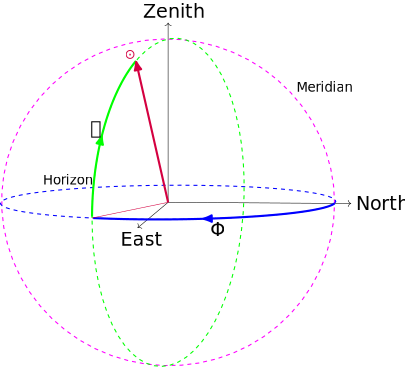
\includegraphics[scale=0.75]{horizontal-coordinate.pdf}
\caption{Horizontal coordinate system}
\label{fig:hz-coordinate}
\end{figure}

In this package, the cardinal points have specifics values of azimuth as following:

\begin{tabular}{c c c c}
North & East & South & West \\
0°    & 90°  & 180°  & 270°
\end{tabular}


The projection of the sun on the horizon plane is a point, which can be defined by two parameters:
\begin{itemize}
\item the angle $\Theta$,
\item the distance $r = \cos(\phi)$ from the centre to the sun.
\end{itemize}

Figure~\ref{fig:sun-projection} shows the projection of the sun on the horizontal plane.
If we track the position of sun on the horizontal plane changes from time to time, we will get a curve.
This curve is called the sun path. 
A chart which shows position of the sun from time to time is called a sun path chart.
Of course there are many type of sun path chart. 
This package provides tools to plot sun path on the horizontal plane.

\begin{figure}[H]
\centering
\begin{tikzpicture}[spradius=3]
\drawcrosshair;
\drawaltitudecircle{{0}}
%\drawazimuthline{{0,10,...,360}}{85}{70}
%\drawazimuthline{{0,5,...,360}}{80}{0}

%\drawazimuthtick

\drawgeodirection
%\drawaltitudelabel{{10,20,...,80,85}}
%\drawazimuthlabel{{0,15,...,350}} ;  

\path[draw=red,fill=red](sunpath cs:azi=110,alt=66) circle[radius=2pt] ;
\end{tikzpicture}
\caption{Projection of the sun on the horizon plane}
\label{fig:sun-projection}
\end{figure}

\subsection{Draw a Sun path chart}

Figure~\ref{fig:sun-projection} is a very rudimentary sun path chart.
There is neither scalar, nor time on the chart. 
A more usable Sun path chart may look like one in the figure~\ref{fig:full-sun-path-chart}.
In this section we will create this chart.


\begin{figure}[H]
\centering
\begin{tikzpicture}
\drawcrosshair
\drawaltitudecircle{{0,10,...,80,85}}
\drawazimuthline{{0,10,...,360}}{85}{70}
\drawazimuthline{{0,5,...,360}}{80}{0}

\drawazimuthtick

\drawgeodirection
\drawaltitudelabel{{10,20,...,80,85}}
\drawazimuthlabel{{0,15,...,350}} ;  

\path[draw=red,fill=red](sunpath cs:azi=110,alt=66) circle[radius=2pt] node[below] {{9:30}};
\end{tikzpicture}
\caption{A Sun path chart}
\label{fig:full-sun-path-chart}
\end{figure}

\subsubsection{Outlines}

The chart is a \TikZ-picture, so we need a \texttt{tikzpicture}-environment.
We can also customize the distance from the centre of the chart to the horizon line by setup the option \texttt{spradius}.
By default it is 5.5 in PGF xy coordinate. 
In this example we make it a little bigger:

\marginpar{\texttt{spradius}}
\begin{verbatim}
\begin{tikzpicture}[spradius=6]
\end{tikzpicture}
\end{verbatim}

We also need the crosshair, the horizon line --in this chart it is a circle--, 
the fours geographic direction.
This can be done by adding more commands into the \texttt{tikzpicture}

\begin{verbatim}
\begin{tikzpicture}[spradius=6]
\drawcrosshair
\drawaltitudecircle{{0}}
\drawgeodirection
\end{tikzpicture}
\end{verbatim}

\marginpar{\texttt{drawcrosshair\\ drawgeodirection\\ drawaltitudecircle}}
\begin{tikzpicture}[spradius=6]
\drawcrosshair
\drawaltitudecircle{{0}}
\drawgeodirection
\end{tikzpicture}


Man has to pay attention to the double curry brackets in the command \texttt{drawaltitudecircle}.
The outer brackets delimit the argument of the command.
The argument of the command is a valid \TikZ-range, which is used in a \verb:\foreach: command,
so it has be placed in between a pair of curry bracket. 
That is the inner brackets.


\subsubsection{Scalar and labels}


As the name of the commando says, we can also draw more than the horizon line by adding some values of altitude in the range of the argument of the command \verb|\drawaltitudecircle|. 
For example \verb:\drawaltitudecircle{{0,10,...,80,85}}: draws 10 circles of altitude.

\begin{verbatim}
\begin{tikzpicture}[spradius=6]
\drawcrosshair
\drawaltitudecircle{{0,10,...,80,85}}
\drawgeodirection
\end{tikzpicture}
\end{verbatim}

\begin{tikzpicture}[spradius=6]
\drawcrosshair
\drawaltitudecircle{{0,10,...,80,85}}
\drawgeodirection
\end{tikzpicture}


We can use the command \verb:\drawazumuthline{r}{h}{l}: to draw azimuth lines in range \verb:r:, 
from the higher altitude \verb:h: to the lower altitude \verb:l:.

For example

\begin{itemize}
  \item \verb:\drawazimuthline{{0,10,...,360}}{85}{70}: draws every 10° azimuth from the 85° altitude to to 70° altitude.
  \item \verb:\drawazimuthline{{0,5,...,360}}{85}{70}: draws every 5° azimuth from the 80° altitude to to 0° altitude.
\end{itemize}

\begin{verbatim}
\begin{tikzpicture}[spradius=6]
\drawcrosshair
\drawaltitudecircle{{0,10,...,80,85}}
\drawazimuthline{{0,10,...,360}}{85}{70}
\drawazimuthline{{0,5,...,360}}{80}{0}

\drawgeodirection
\end{tikzpicture}
\end{verbatim}

\marginpar{\texttt{drawazimuthline}}
\begin{tikzpicture}[spradius=6]
\drawcrosshair
\drawaltitudecircle{{0,10,...,80,85}}
\drawazimuthline{{0,10,...,360}}{85}{70}
\drawazimuthline{{0,5,...,360}}{80}{0}

\drawgeodirection
\end{tikzpicture}
















